\documentclass[a4paper,10pt]{article}
\usepackage[utf8]{inputenc}
\usepackage{graphicx}
\begin{document}
\begin{figure}[ht]
 \centering
\begin{minipage}[c]{0.45\textwidth}
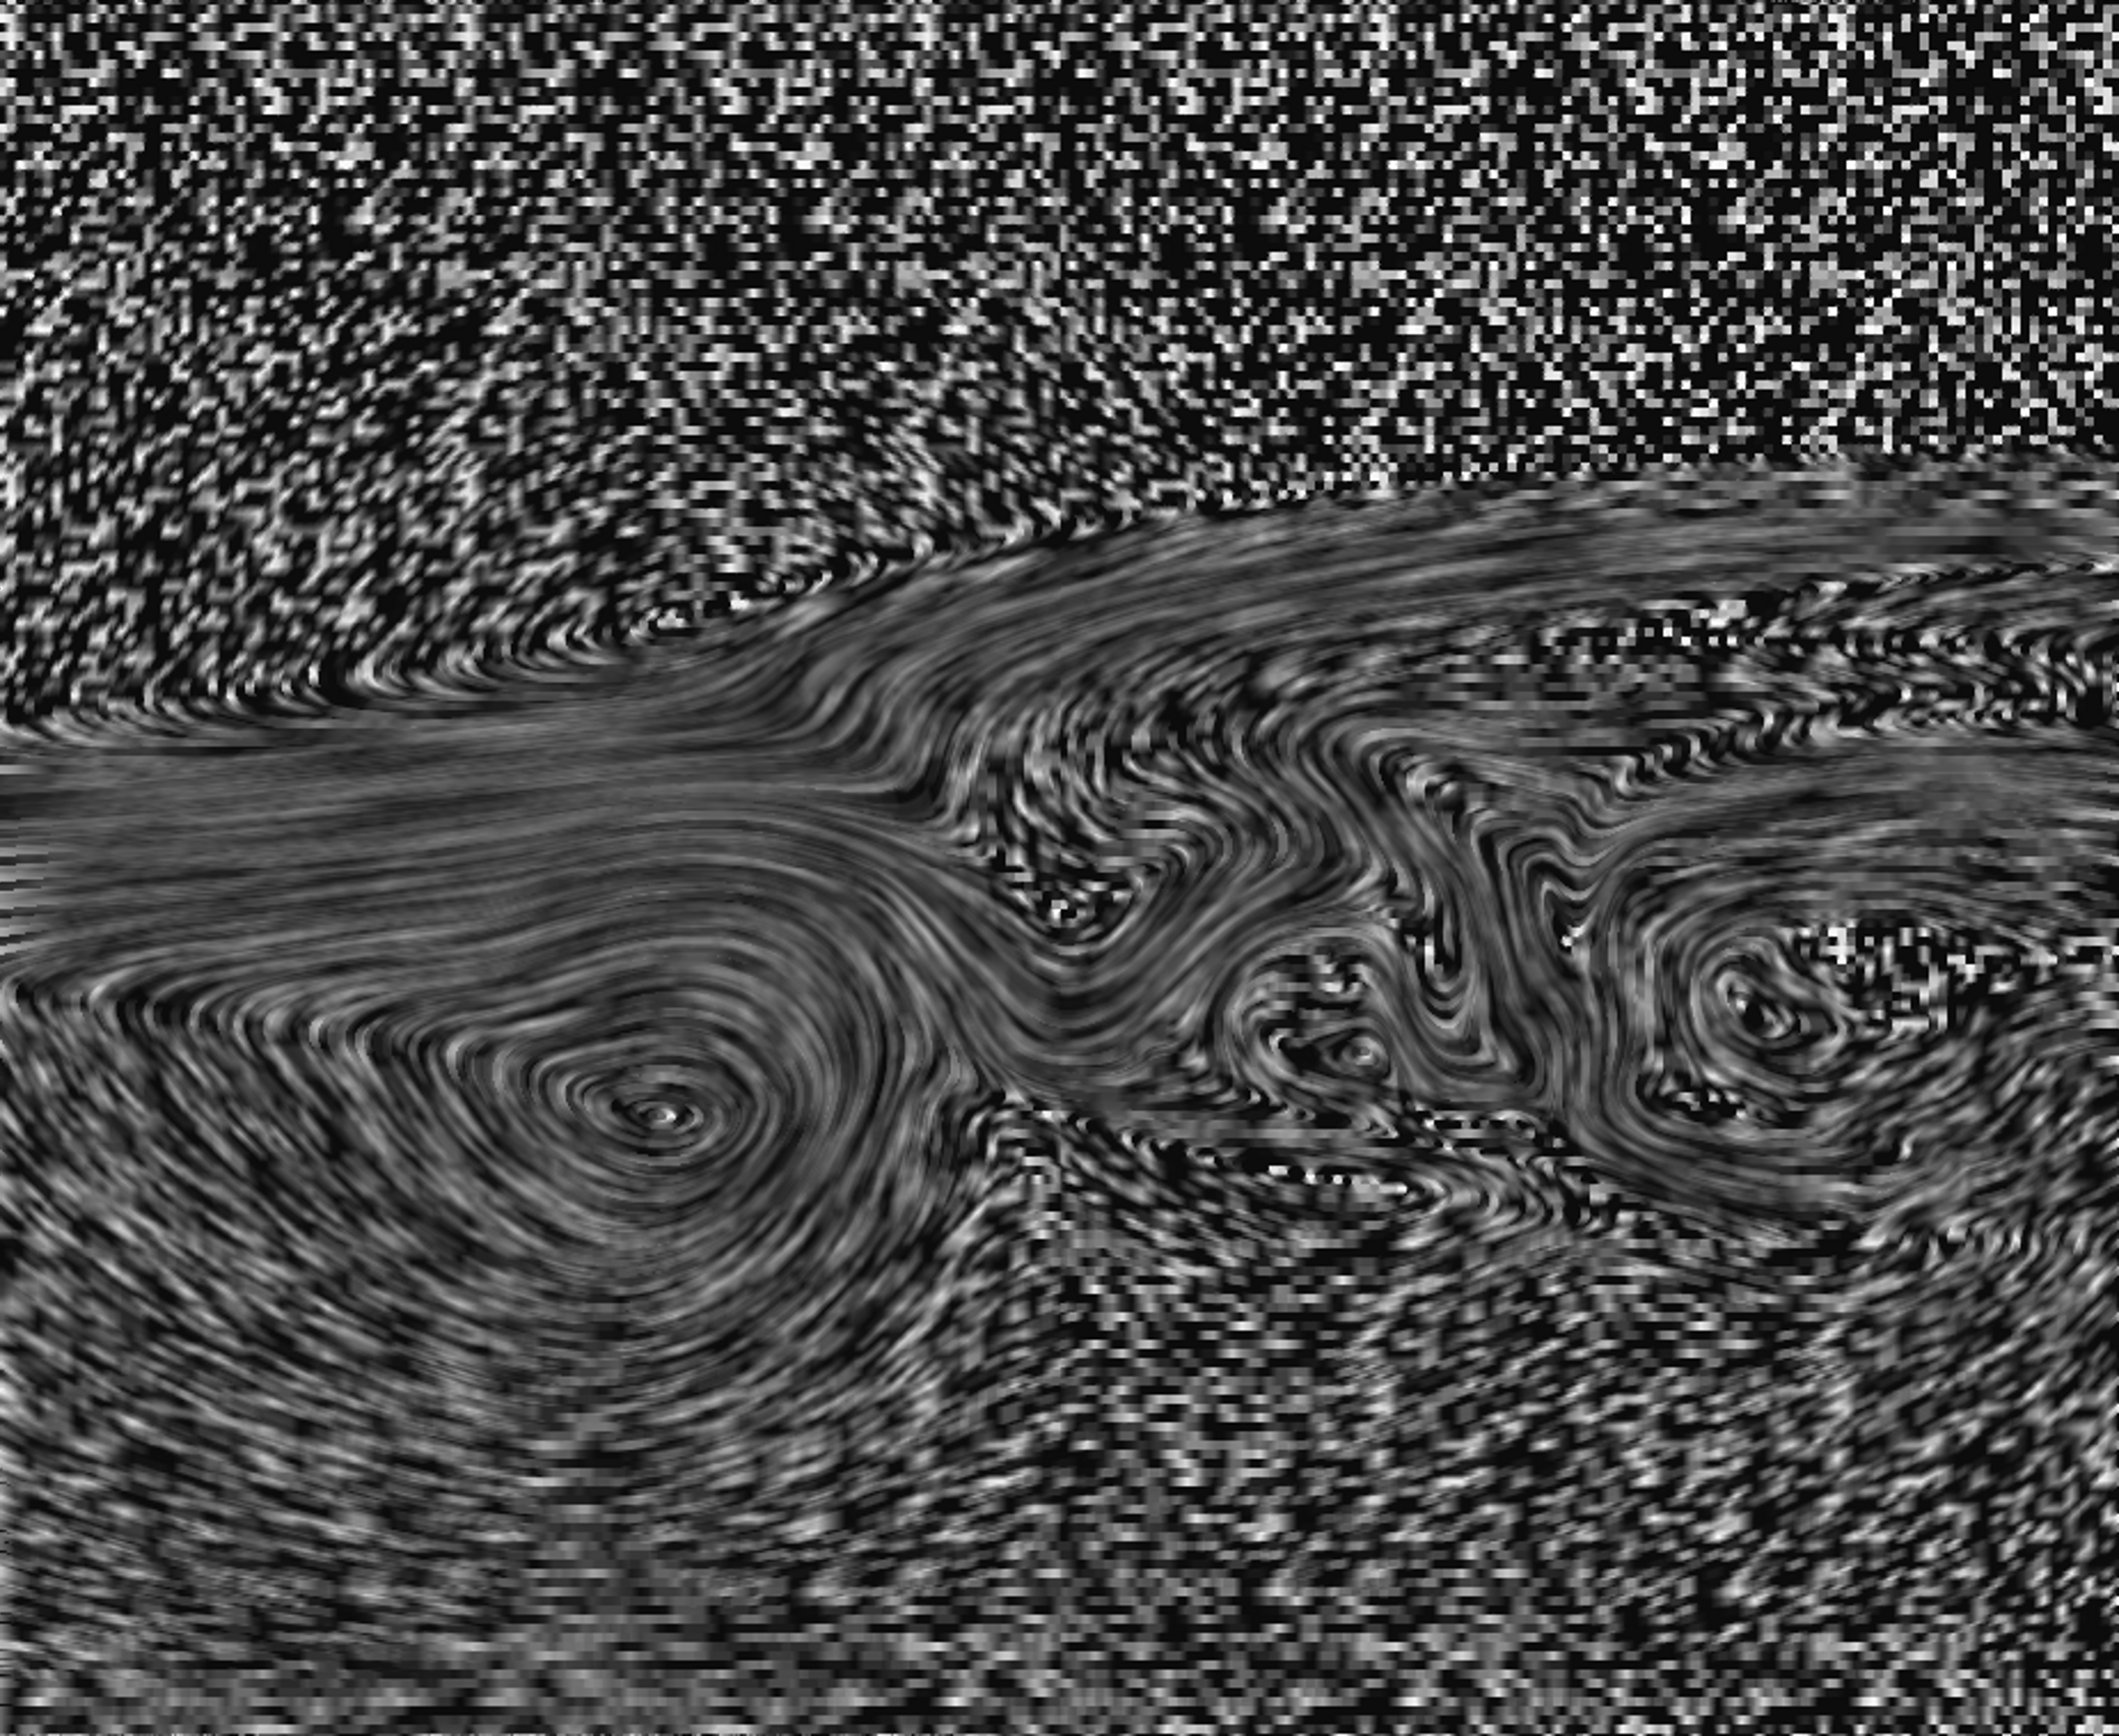
\includegraphics[width=\textwidth]{asym-2d-bw-no-norm.png}
\end{minipage}\hspace{0.1in}
% \begin{minipage}[t]{0.3\textwidth}
% 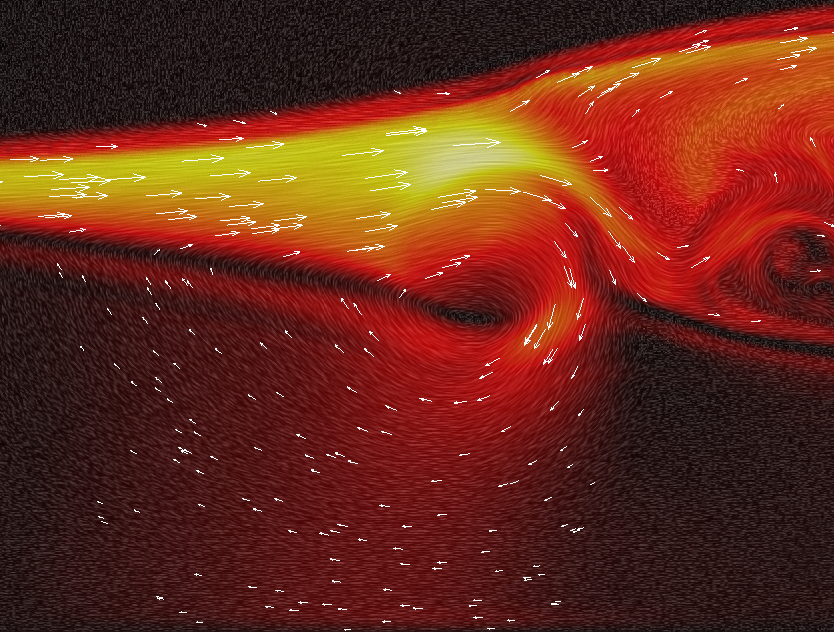
\includegraphics[width=\textwidth]{2d-asym-with-glyphs-crop.png}
% \end{minipage}
\begin{minipage}[c]{0.45\textwidth}
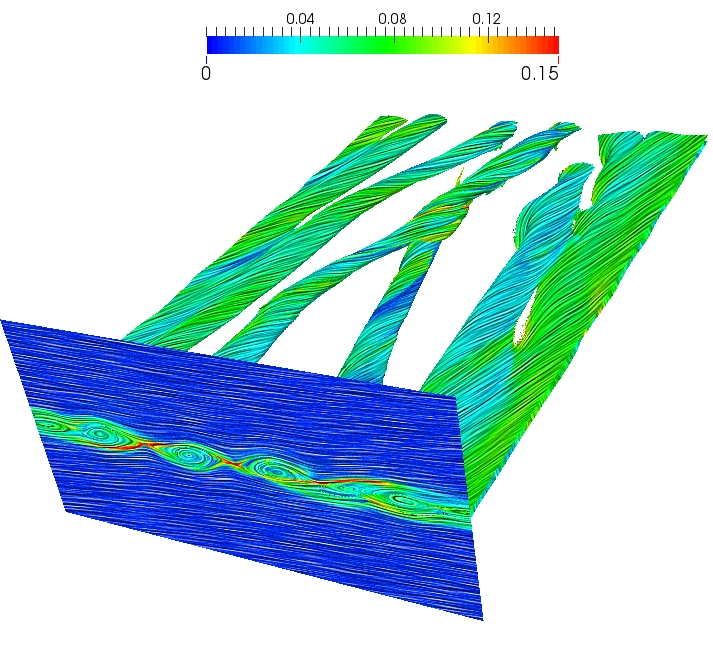
\includegraphics[width=\textwidth]{flux-ropes.png}
\end{minipage}
 \caption{example LIC figures}
 \label{fig:LIC}
\end{figure}
\section{LIC}
The standard way to visualize streamlines of a vector field is to seed some points and integrate to trace curves that are instantaneously tangent to the velocity vector. Although useful, this approach can be cumbersome when interactively exploring a dataset. For example, the technique is inherently local and unless feature locations are know apriori it's difficult to select an effective set of seed points. An alternative technique called ”line integral convolution” or LIC, which convolves noise with a vector field producing streaking patterns that follow vector field tangents, has the advantage that a very detailed view of the streamlines over the entire computational domain is found in one step without the need to explicitly specify a set of seed points. The technique was initially developed for use on images\cite{LIC1}, but has since been extended to arbitrary surfaces\cite{LIC2}, and to volumes as well\cite{LIC3}. The algorithm has been ported to the GPU\cite{LIC5} and data-parallel implementations have been developed\cite{LIC4}. The results in this paper were produced using ParaView\cite{PV}, an open source , cross platform, tool for parallel  interactive visualization of large datasets. In addition to traditional visualization algorithms ParaView provides an MPI based data-parallel GP-GPU surface LIC algorithm which includes a number of enhancements to the basic LIC algorithm designed for interactive data exploration. ParaView's surface LIC can be used on massive super computers with our without GPUs. It's described in detail in ParaView's online documentation\cite{PV2}. To aid the reader in the interpretation of the figures presented here a brief review of the LIC algorithm is presented here.

The LIC algorithm of a vector field defined on an image, $I(x,y)$, is given by the following integral over streamline arcs computed from the center of each pixel location, $x,y$.
\begin{equation}
 I(x,y) = \frac{\displaystyle \int_{-L}^{L} k(i)N(S_i)di}{\displaystyle \int_{-L}^{L} k(i) di}
\end{equation}
where $L$ is the integration length, $N$ generates the noise value at a given location, $S_i$ is a position on a streamline arc centered at $x,y$, $k(i)$ is an approriate convolution kernel, and $I(x,y)$ is the image  pixel at $x,y$. In practice streamline arcs are computed using an RK method over a fixed number of steps, and $L$ may be a constant for all pixels in $I$, or it may be a function of the local vector field. When $L$ is constant the resulting visualization has a uniform look. When $L$ varies as a function of the vector local field the visualzaiton accurately shows relative strengths of flow features. Because the LIC produces a dense representation of the flow field, features of interest can be quickly identified. LIC is often used in conjunction with scalar pseudocoloring. In this case a specialized shader is used to combine the colors with the gray scale LIC image. Optimized implementations, especially data-parallel or GPU based, are very fast making the technique useful for interactive data exploration. An example of image LIC is shown in the left panel of figure \ref{fig:LIC}. The surface LIC technique we use is similar to image based LIC except first vectors are projected onto the surface then into image space where an image LIC algorithm is used to compute LIC\cite{LIC2}. Lit, pseudocolored surface geometry is combined with the image LIC to produce a realistic rendering of the surface geometry. An example of surface LIC on isocontour of density in VPIC plasma simulation is shown in right panel of figure \ref{fig:LIC}.
\end{document}
